\documentclass[a4paper,11pt]{article}

%\usepackage[T1]{fontenc}
\usepackage[swedish]{babel}
%\usepackage[utf8]{inputenc}
\usepackage{graphicx}
\usepackage{sidecap}
\usepackage{listings}
\usepackage[a4paper]{geometry}
\usepackage{fontspec}
\usepackage{fancyhdr}
\usepackage{pdfpages}
\usepackage{hyperref}


\lstset{
	language=C,
	numbers=left,
	numberstyle=\tiny,
	numbersep=8pt,
	basicstyle=\ttfamily\footnotesize,
	commentstyle=\small,
	keywordstyle=\bfseries,
	stringstyle=\ttfamily,
	showstringspaces=true,
	breaklines=true,
	tabsize=4,
	frame=none,
	title=\lstname
}

\providecommand*\email[1]{\it \href{mailto:#1}{#1}}

\setcounter{secnumdepth}{0}
\setlength{\parindent}{0pt}
\setlength{\parskip}{2ex}


\pagestyle{fancy}
\fancyhead{}
%\fancyhead[RO,RE]{Mattis Kancans Envall, \emph{mattiske@kth.se}}
%\fancyhead[LO,LE]{pallinda13}
%\renewcommand{\headrulewidth}{0.4pt}
%\renewcommand{\footrulewidth}{0.4pt}

\author{Simon Ström\\\email{simstr@kth.se}\\Mattis Kancans Envall\\\email{mattiske@kth.se}}
\title{ID2200 Operativsystem\\ Lab 1: Kommunikation med pipes }

\begin{document}
    \includepdf[pages={5}]{../LabPm.pdf}
    %\maketitle

    \section{Kommunikation med pipes}
        \subsection{Uppgiften}
        Uppgiften är att skriva ett program som låter användaren studera sina miljövariabler. Vid exekvering skall programmet visa samtliga miljövariabler, i bokstavsordnig. Dessutom skall användaren kunna filtrera resultatet med samma syntax som ett anrop till {\tt grep} skulle innebära.
        \subsection{Vår lösning}
        Vi har löst detta genom att låta programmet förgrena sig medhjälp av sk.{\it forks}, vilket i praktiken innebär att nya instanser av programmet körs som barnprocesser. Hur programmet förgrenas syns i Figur ~\ref{fig:processtree}:
\begin{figure}[h!]
  \centering
  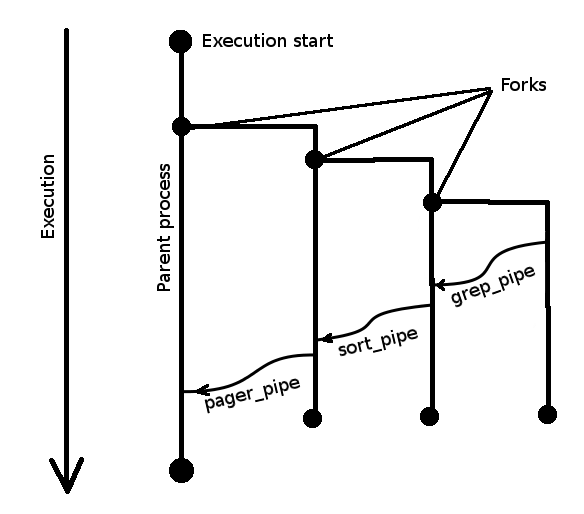
\includegraphics[scale=0.3]{imgs/fig1.png}
  \caption{Processträd}
  \label{fig:processtree}
\end{figure}

Barnprocesserna kommer i sin tur att producera och skicka resultatet från {\tt printenv}, {\tt grep}, {\tt sort} och {\tt less} (om inte annan pager är satt) på motsvarande pipes. Detta betyder att det första barnet kommer starta nästa barn, och först när resultatet från denna process finns tillgängligt, kommer barnet köra sitt kommando. Detta betyder att det är enkelt att lägga till fler kommandon ifall detta önskas.



\end{document}
